\documentclass{article}
\usepackage{amsmath, amssymb}
\usepackage{tikz}

\begin{document}

\begin{figure}[h]
    \centering
    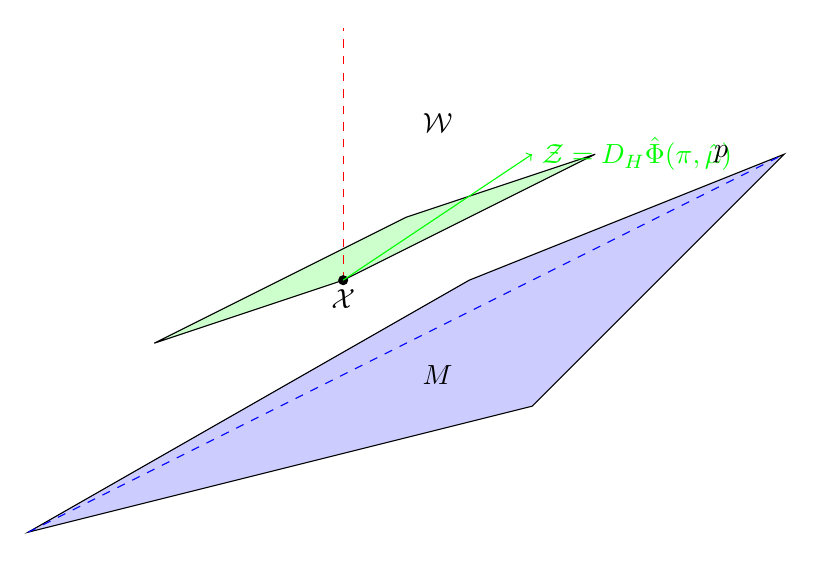
\begin{tikzpicture}[scale=0.8]
        % Draw the shaded region labeled as $\mathcal{B}$
        \filldraw[fill=blue!20] (-3,-3) -- (4,1) -- (9,3) -- (5,-1) -- cycle;
        
        % Draw the dashed line representing the tangent space $T_H \mathcal{B}$
        \draw[dashed, blue] (-3,-3) -- (9,3);
        
        % Draw the solid green region labeled as $\mathcal{Y} = \Psi(\xi,w)$
        \filldraw[fill=green!20] (-1,0) -- (3,2) -- (6,3) -- (2,1) -- cycle;
        
        % Draw the dashed line representing the wave set $\mathcal{W}$
        \draw[dashed, red] (2,1) -- (2,5);
        
        % Draw the solid black point labeled as $\mathcal{X}$
        \filldraw[black] (2,1) circle (2pt) node[below] {$\mathcal{X}$};
        
        % Draw the solid green arrow representing $\mathcal{Z} = D_H \hat{\Phi}(\pi,\hat{\mu})$
        \draw[->, green] (2,1) -- (5,3) node[right] {$\mathcal{Z} = D_H \hat{\Phi}(\pi,\hat{\mu})$};
        
        % Label the point where $\mathcal{W}$ intersects the green region
        \node at (3.5, 3.5) {$\mathcal{W}$};
        \node at (3.5, -0.5) {$M$};
        \node at (8, 3) {$p$};
    \end{tikzpicture}
    \caption{Depiction of Lemma~\ref{lemma:orthog_wave_and_balanced_set}: the wave set is $L^2_H$--orthogonal to the formal tangent space to the balanced set.}
    \label{fig:orthog_wave_and_balanced_set}
\end{figure}

\end{document}